% SFM, GNM: 
% - RiMEA 1
% - RiMEA 6
% - Chicken Test
% --> observations
% --> differences, similarities between models
% --> reason for behavior?
In the second task, the same scenarios are used, however, two different models are considered together with the OSM. 
\begin{itemize}
    \item Social Force Model (SFM): 
"It is suggested that the motion of pedestrians can be described as if they would be subject to `social forces'. These `forces' are not directly exerted by the pedestrians' personal environment, but they are a measure for the internal motivations of the individuals to perform certain actions (movements)." \cite{Helbing_1995}\\ 
    \item Gradient Navigation Model (GNM): 
"The model uses a superposition of gradients of distance functions to directly change the direction of the velocity vector. The velocity is then integrated to obtain the location." \cite{Dietrich_2014}
\end{itemize}

\textbf{RiMEA scenario 1 (straight line):}\\
For the SFM, pedestrians move closer together compared to OSM. The degree of compaction is distinctly higher: we can distinguish one single lane in the center of the corridor. That  is not the case for the OSM for which the movement seems more disorganized. 
%%%%%%%%%%%%%%%%%%%%%%%%%%%%%
The GNM looks the most different compared to the two above. Pedestrians split into three distinctive rows and move along a grid, sometimes changing lanes. This model is the one that makes the movement here the most "organized". 
%%%%%%%%%%%%%%%%%%%%%%5

\begin{figure}[H]
 \centering
 \begin{subfigure}[b]{0.6\textwidth}
     \centering
     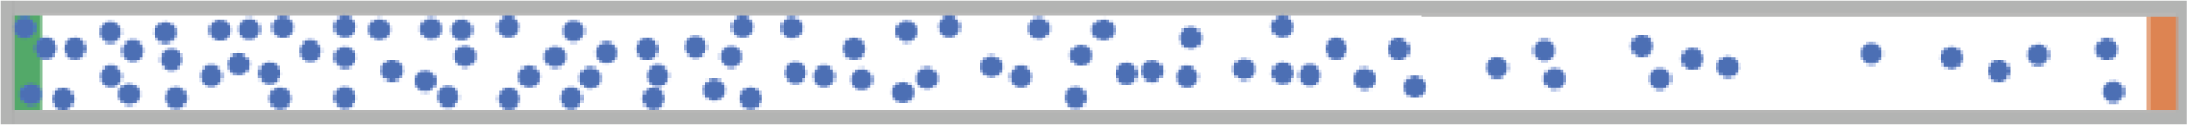
\includegraphics[width=\textwidth]{images/2-osm-rimea1.png}
    \caption{Optimal Step Model}
    \label{fig: rimea1-osm}
 \end{subfigure}
 \begin{subfigure}[b]{0.6\textwidth}
      \centering
     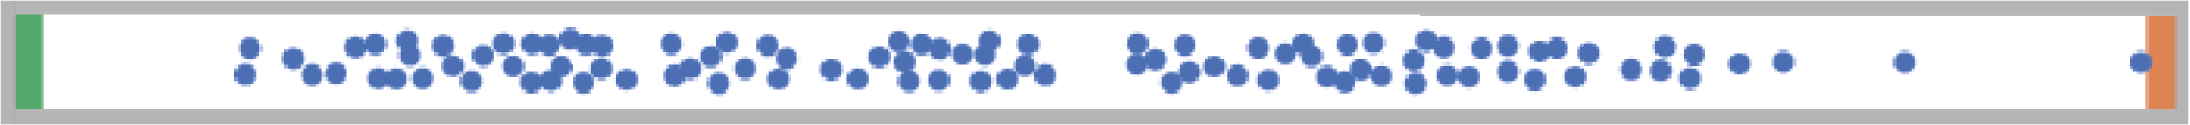
\includegraphics[width=\textwidth]{images/2-sfm-rimea1.png}
     \caption{Social Force Model}
     \label{fig: rimea1-sfm}
 \end{subfigure}
 \begin{subfigure}[b]{0.6\textwidth}
      \centering
     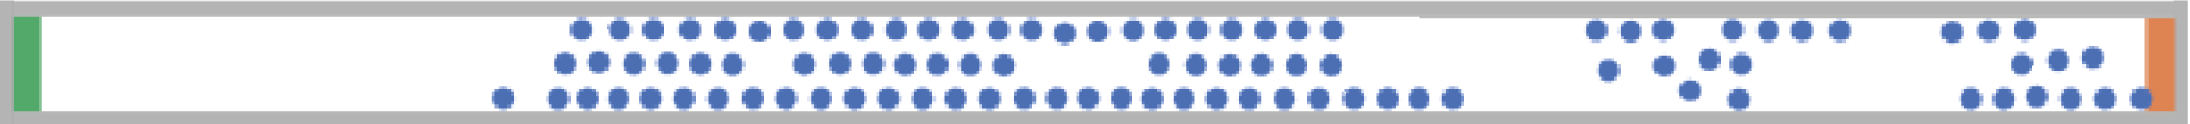
\includegraphics[width=\textwidth]{images/2-gnm-rimea1.png}
     \caption{Gradient Navigation Model}
     \label{fig: rimea1-gnm}
 \end{subfigure}
 \caption{RiMEA Scenario 1 using different models}
 \label{fig: rimea1}
\end{figure}

\textbf{RiMEA scenario 6 (movement around a corner):}\\
When moving around a corner, pedestrians behave in distinct ways for each of the models. In the OSM, they are spread out and move evenly toward the target. The SFM shows the pedestrians walking close to the middle of the corridor, whereas in the GNM, they move close to the wall, taking the shortest way to the target. Both of these models however do not make good use of the available space and therefore look less natural compared to the OSM. 

\begin{figure}[H]
 \centering
 \begin{subfigure}[b]{0.3\textwidth}
     \centering
     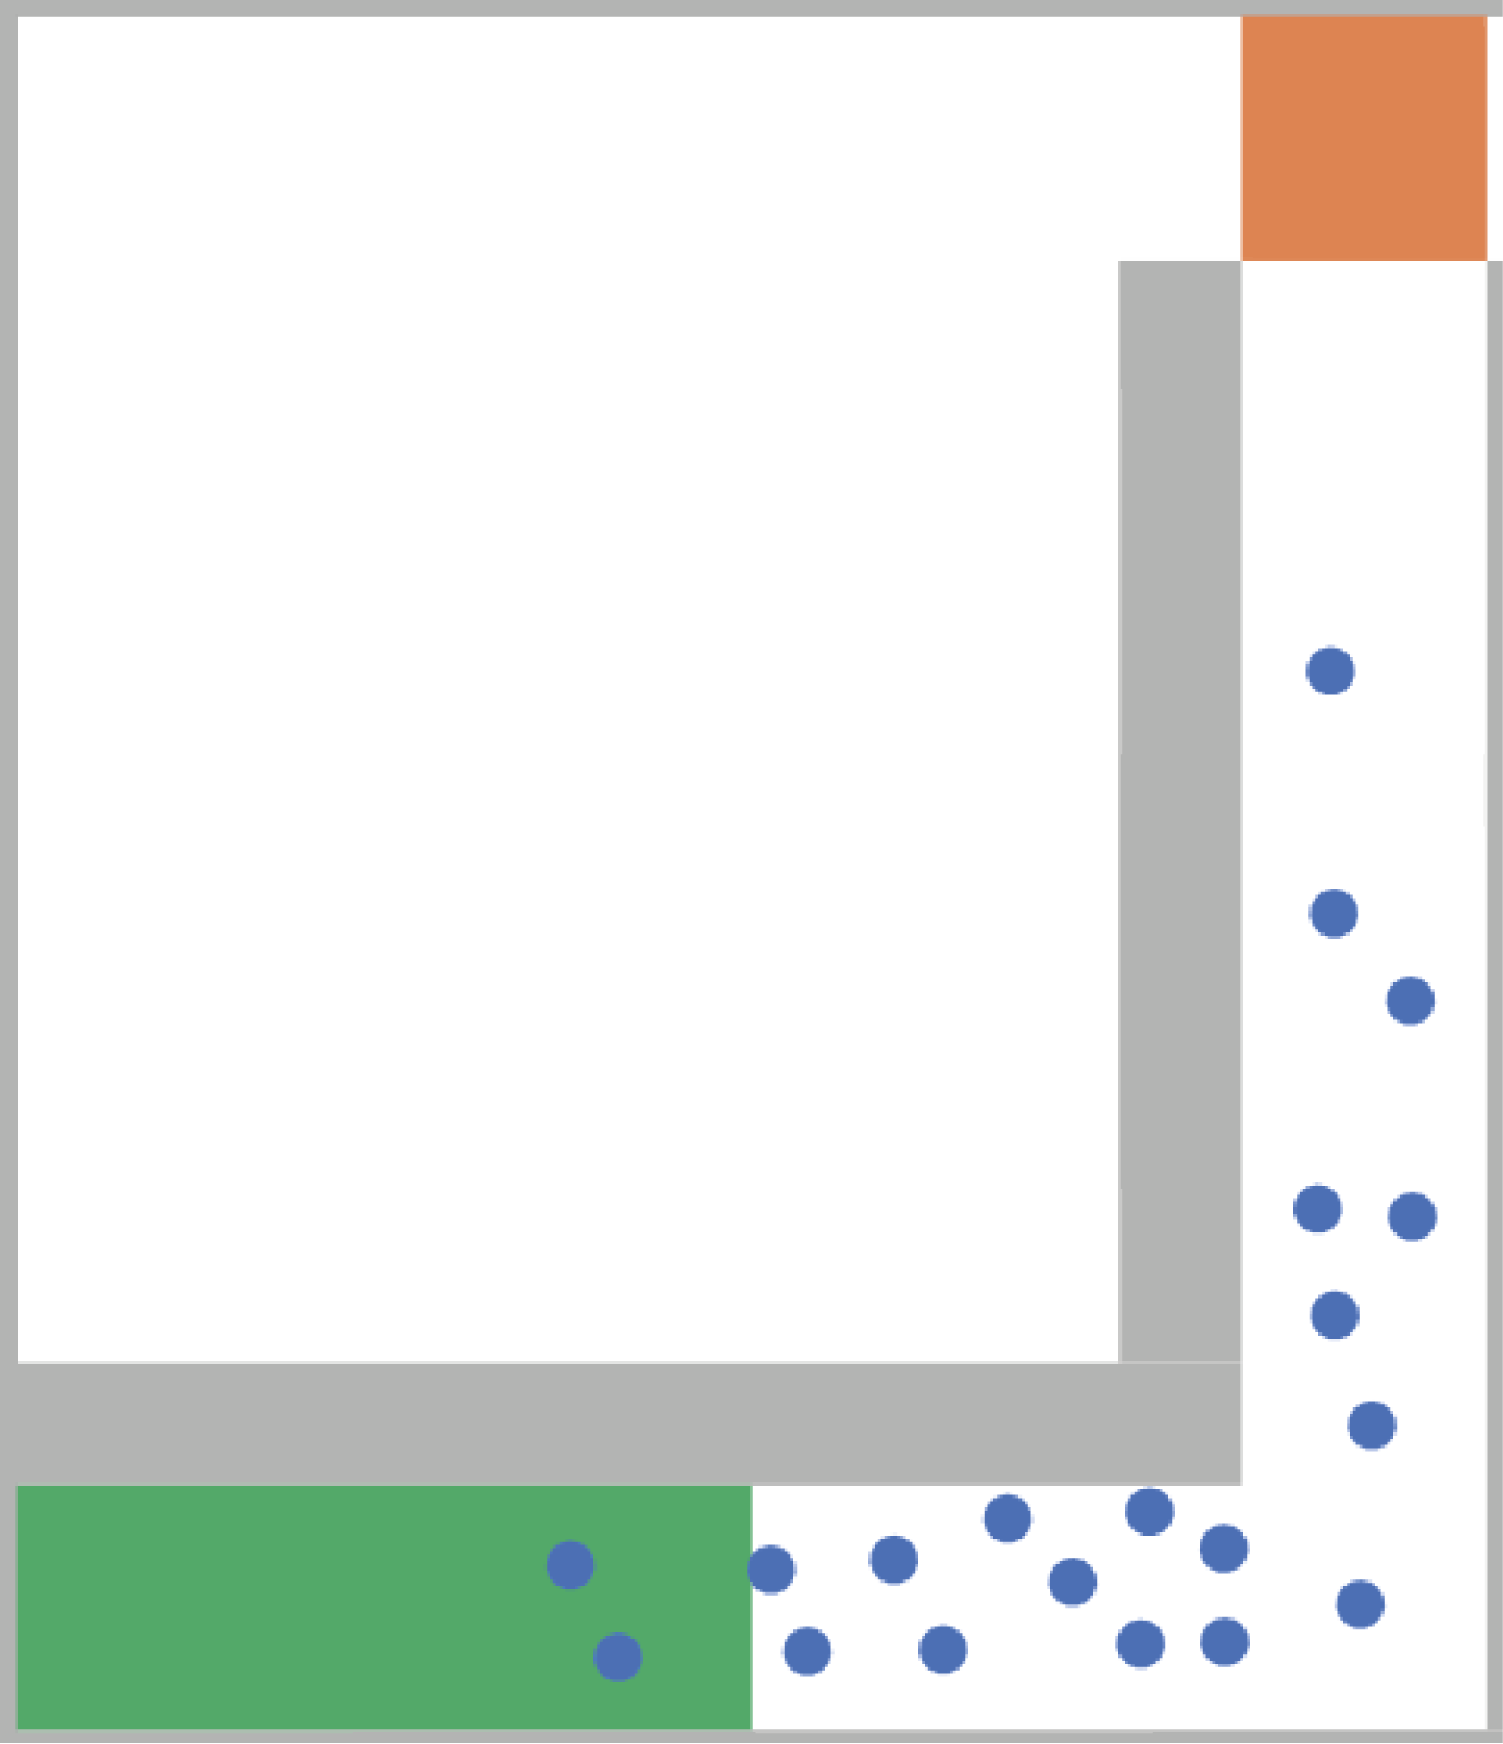
\includegraphics[width=\textwidth]{images/2-osm-rimea6.png}
    \caption{Optimal Step Model}
    \label{fig: rimea6-osm}
 \end{subfigure}
 \begin{subfigure}[b]{0.3\textwidth}
      \centering
     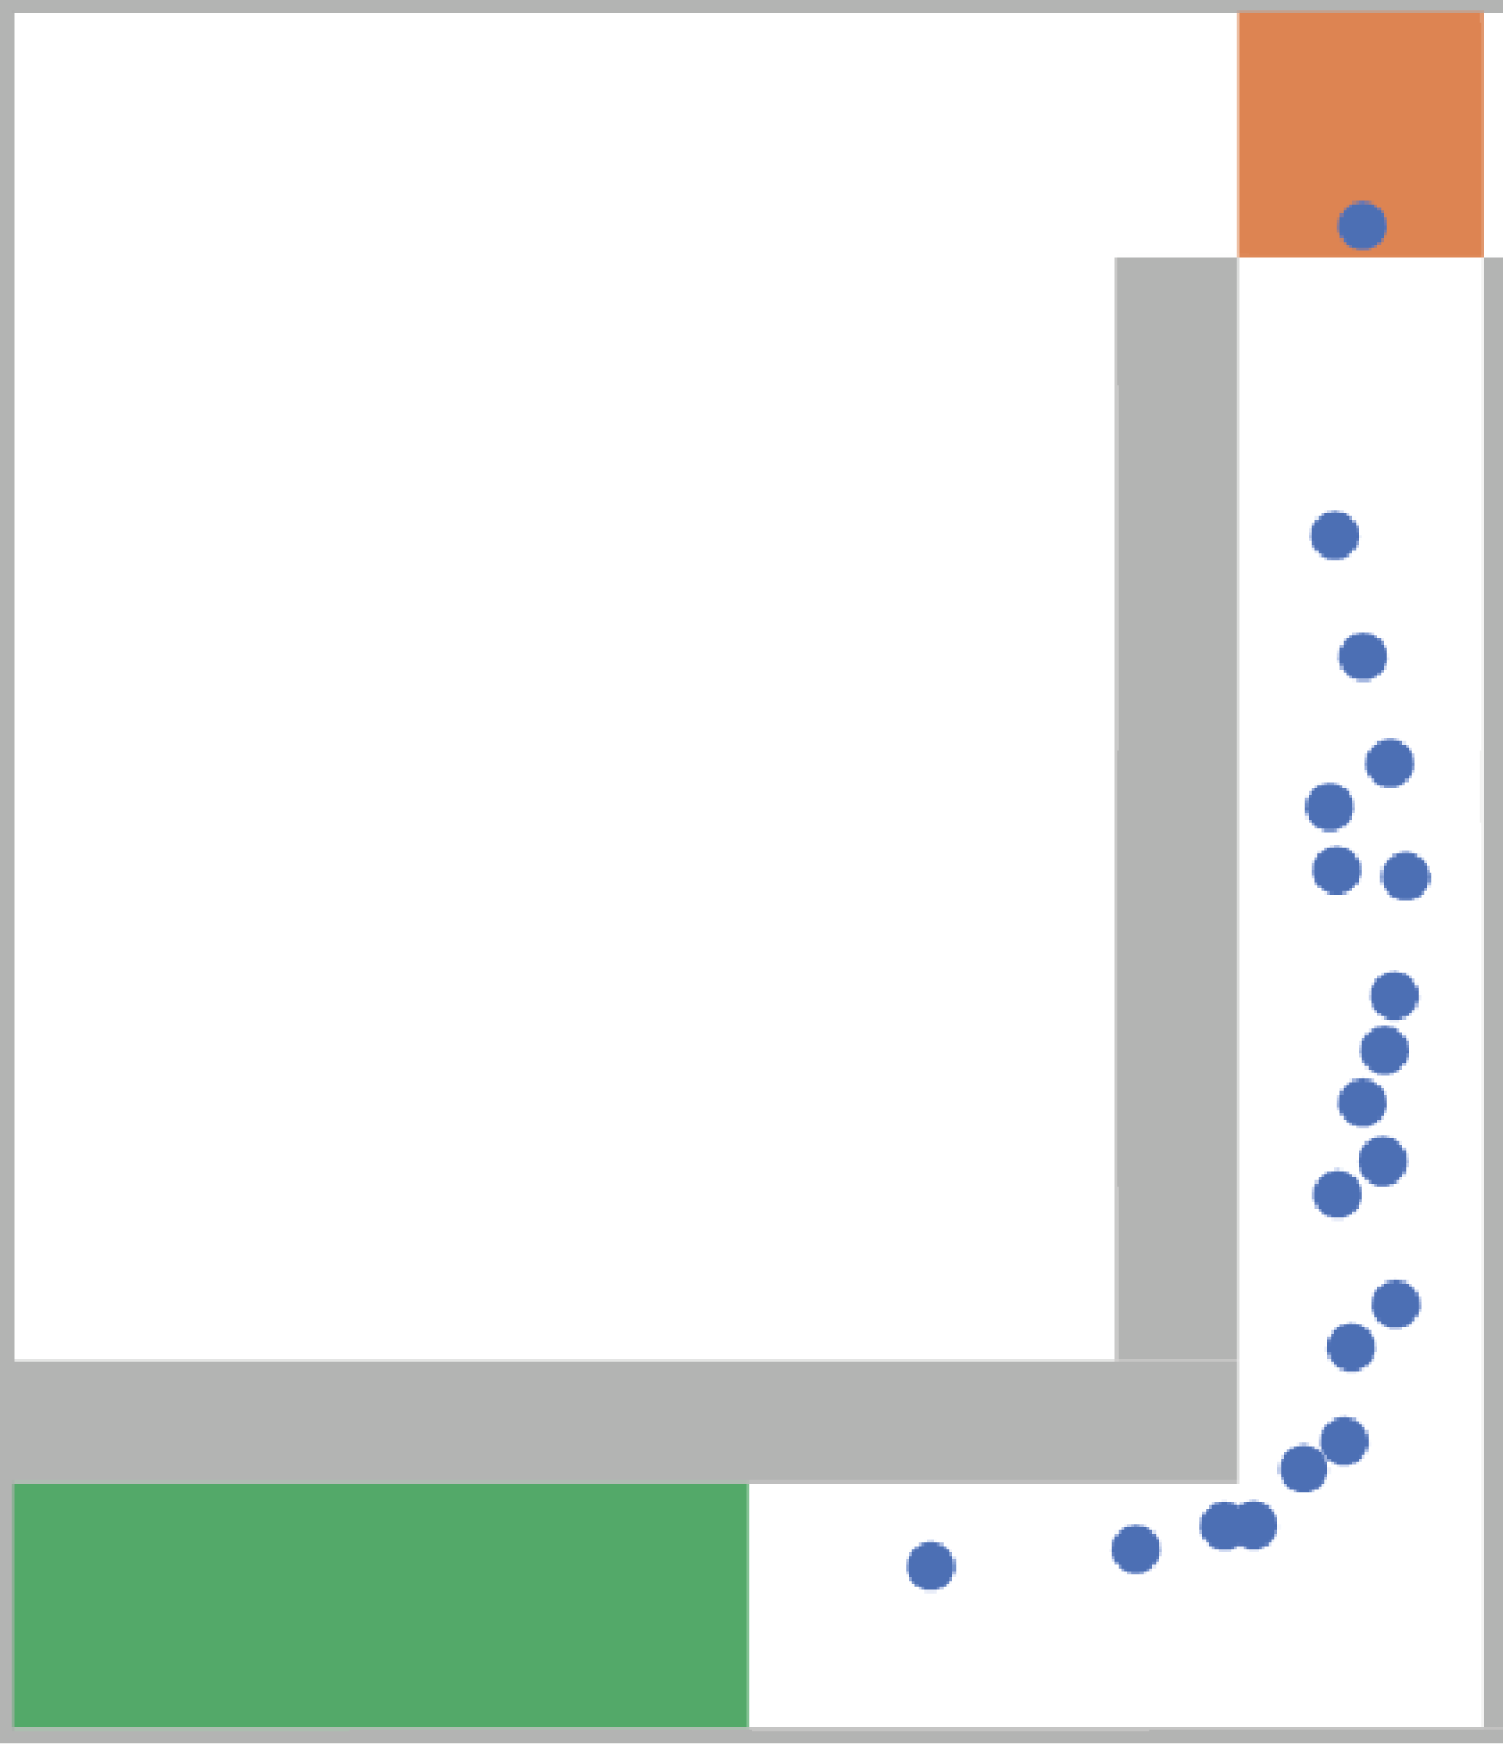
\includegraphics[width=\textwidth]{images/2-sfm-rimea6.png}
     \caption{Social Force Model}
     \label{fig: rimea6-sfm}
 \end{subfigure}
 \begin{subfigure}[b]{0.3\textwidth}
      \centering
     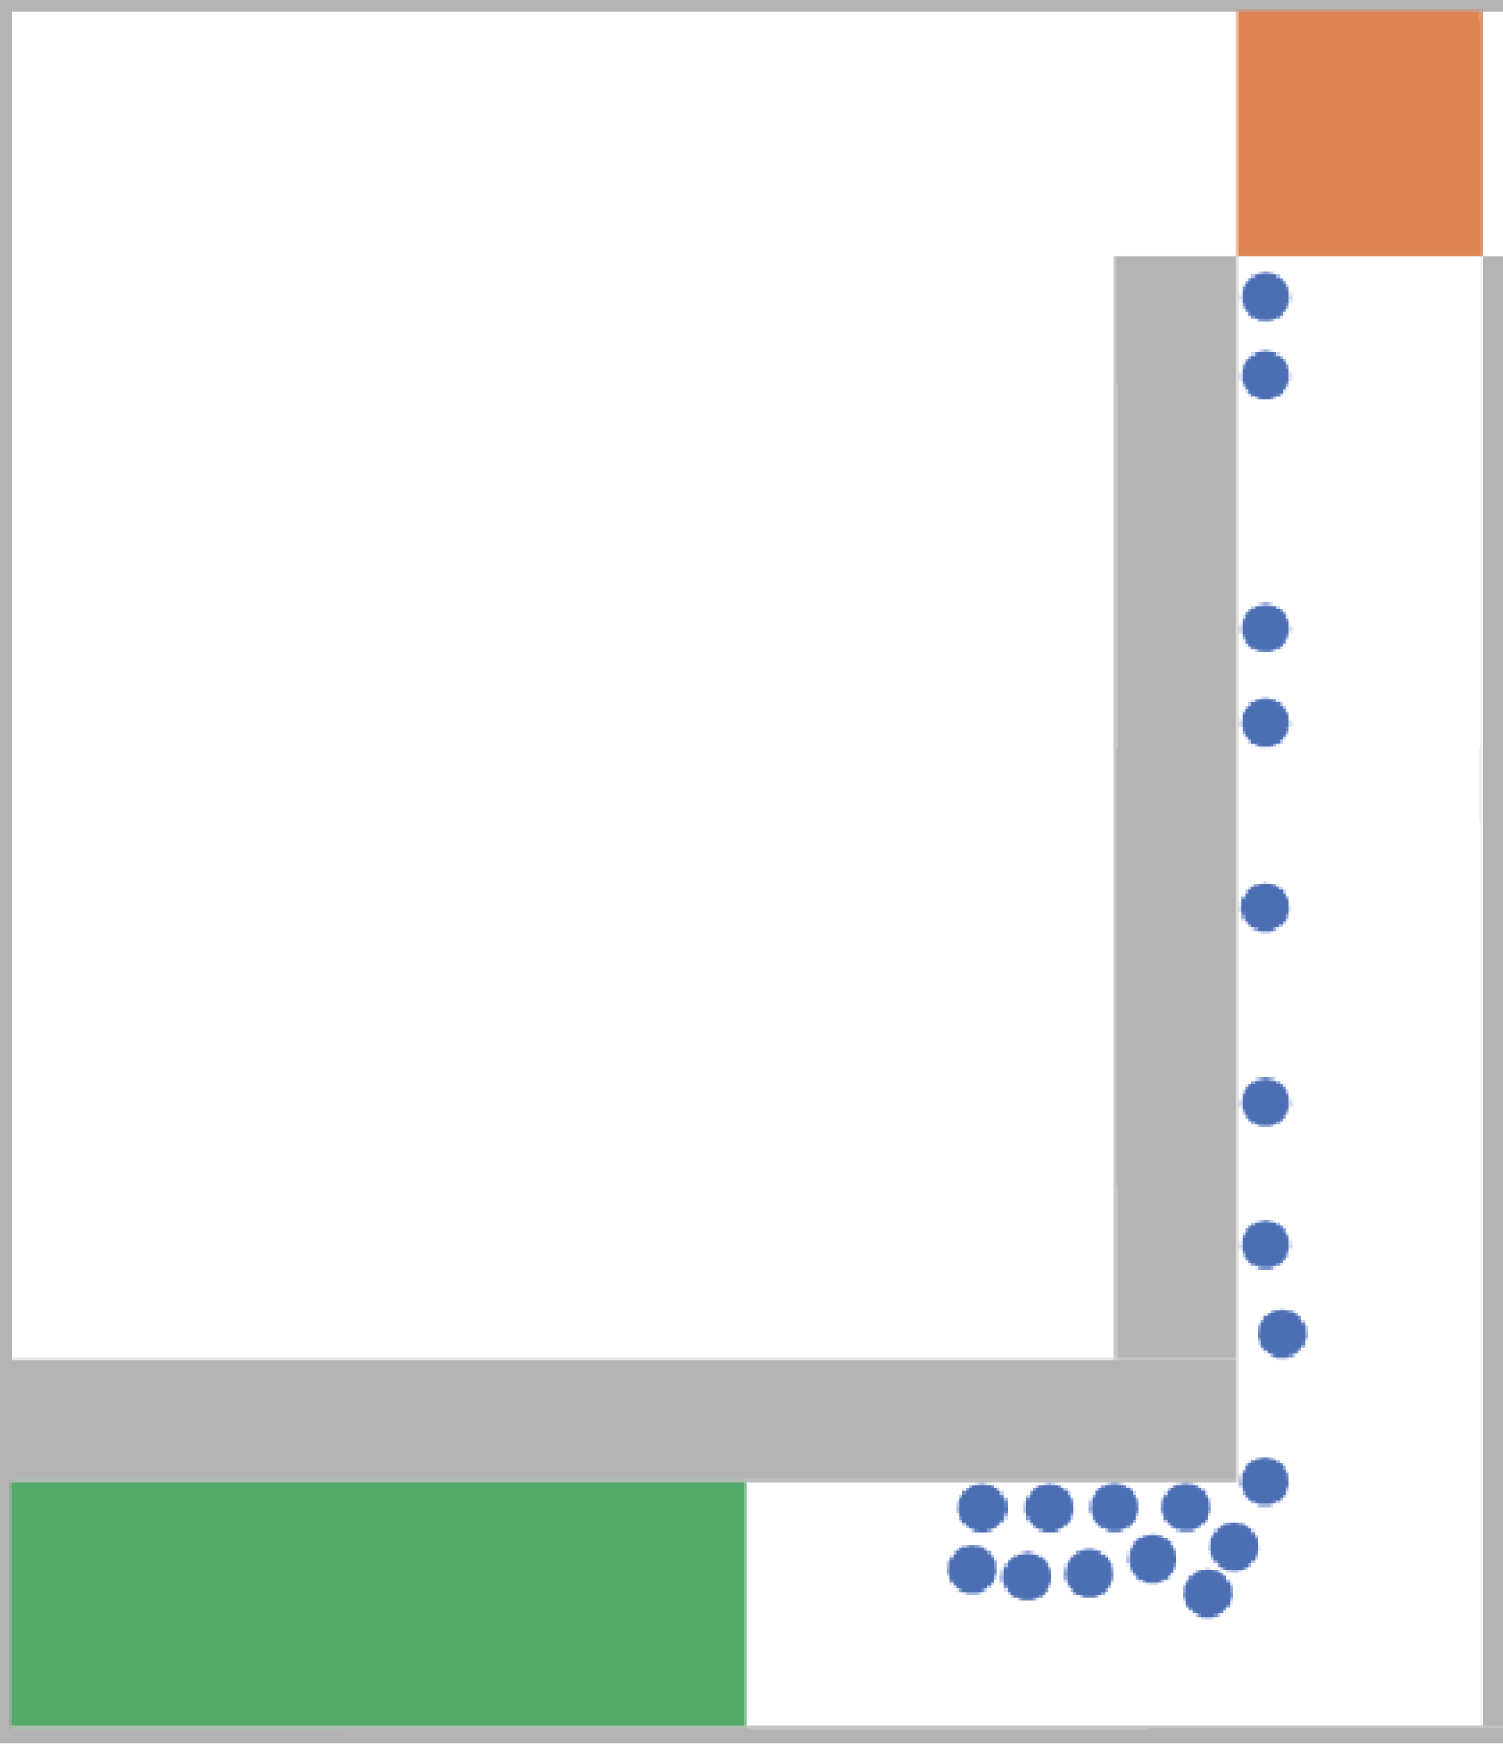
\includegraphics[width=\textwidth]{images/2-gnm-rimea6.png}
     \caption{Gradient Navigation Model}
     \label{fig: rimea6-gnm}
 \end{subfigure}
 \caption{RiMEA Scenario 6 using different models}
 \label{fig: rimea6}
\end{figure}

\textbf{Chicken Test:}\\
All three of the models successfully pass the chicken test. However, differences in the pedestrian's movements can still be observed. The pedestrian in the OSM moves in an angular pattern around the obstacle. In the SFM, the pedestrian moves more naturally, leaving space between the obstacle and its walking path. The GNM shows similar behavior but leaves merely any space in between the wall and the pedestrian. 

\begin{figure}[H]
 \centering
 \begin{subfigure}[b]{0.3\textwidth}
     \centering
     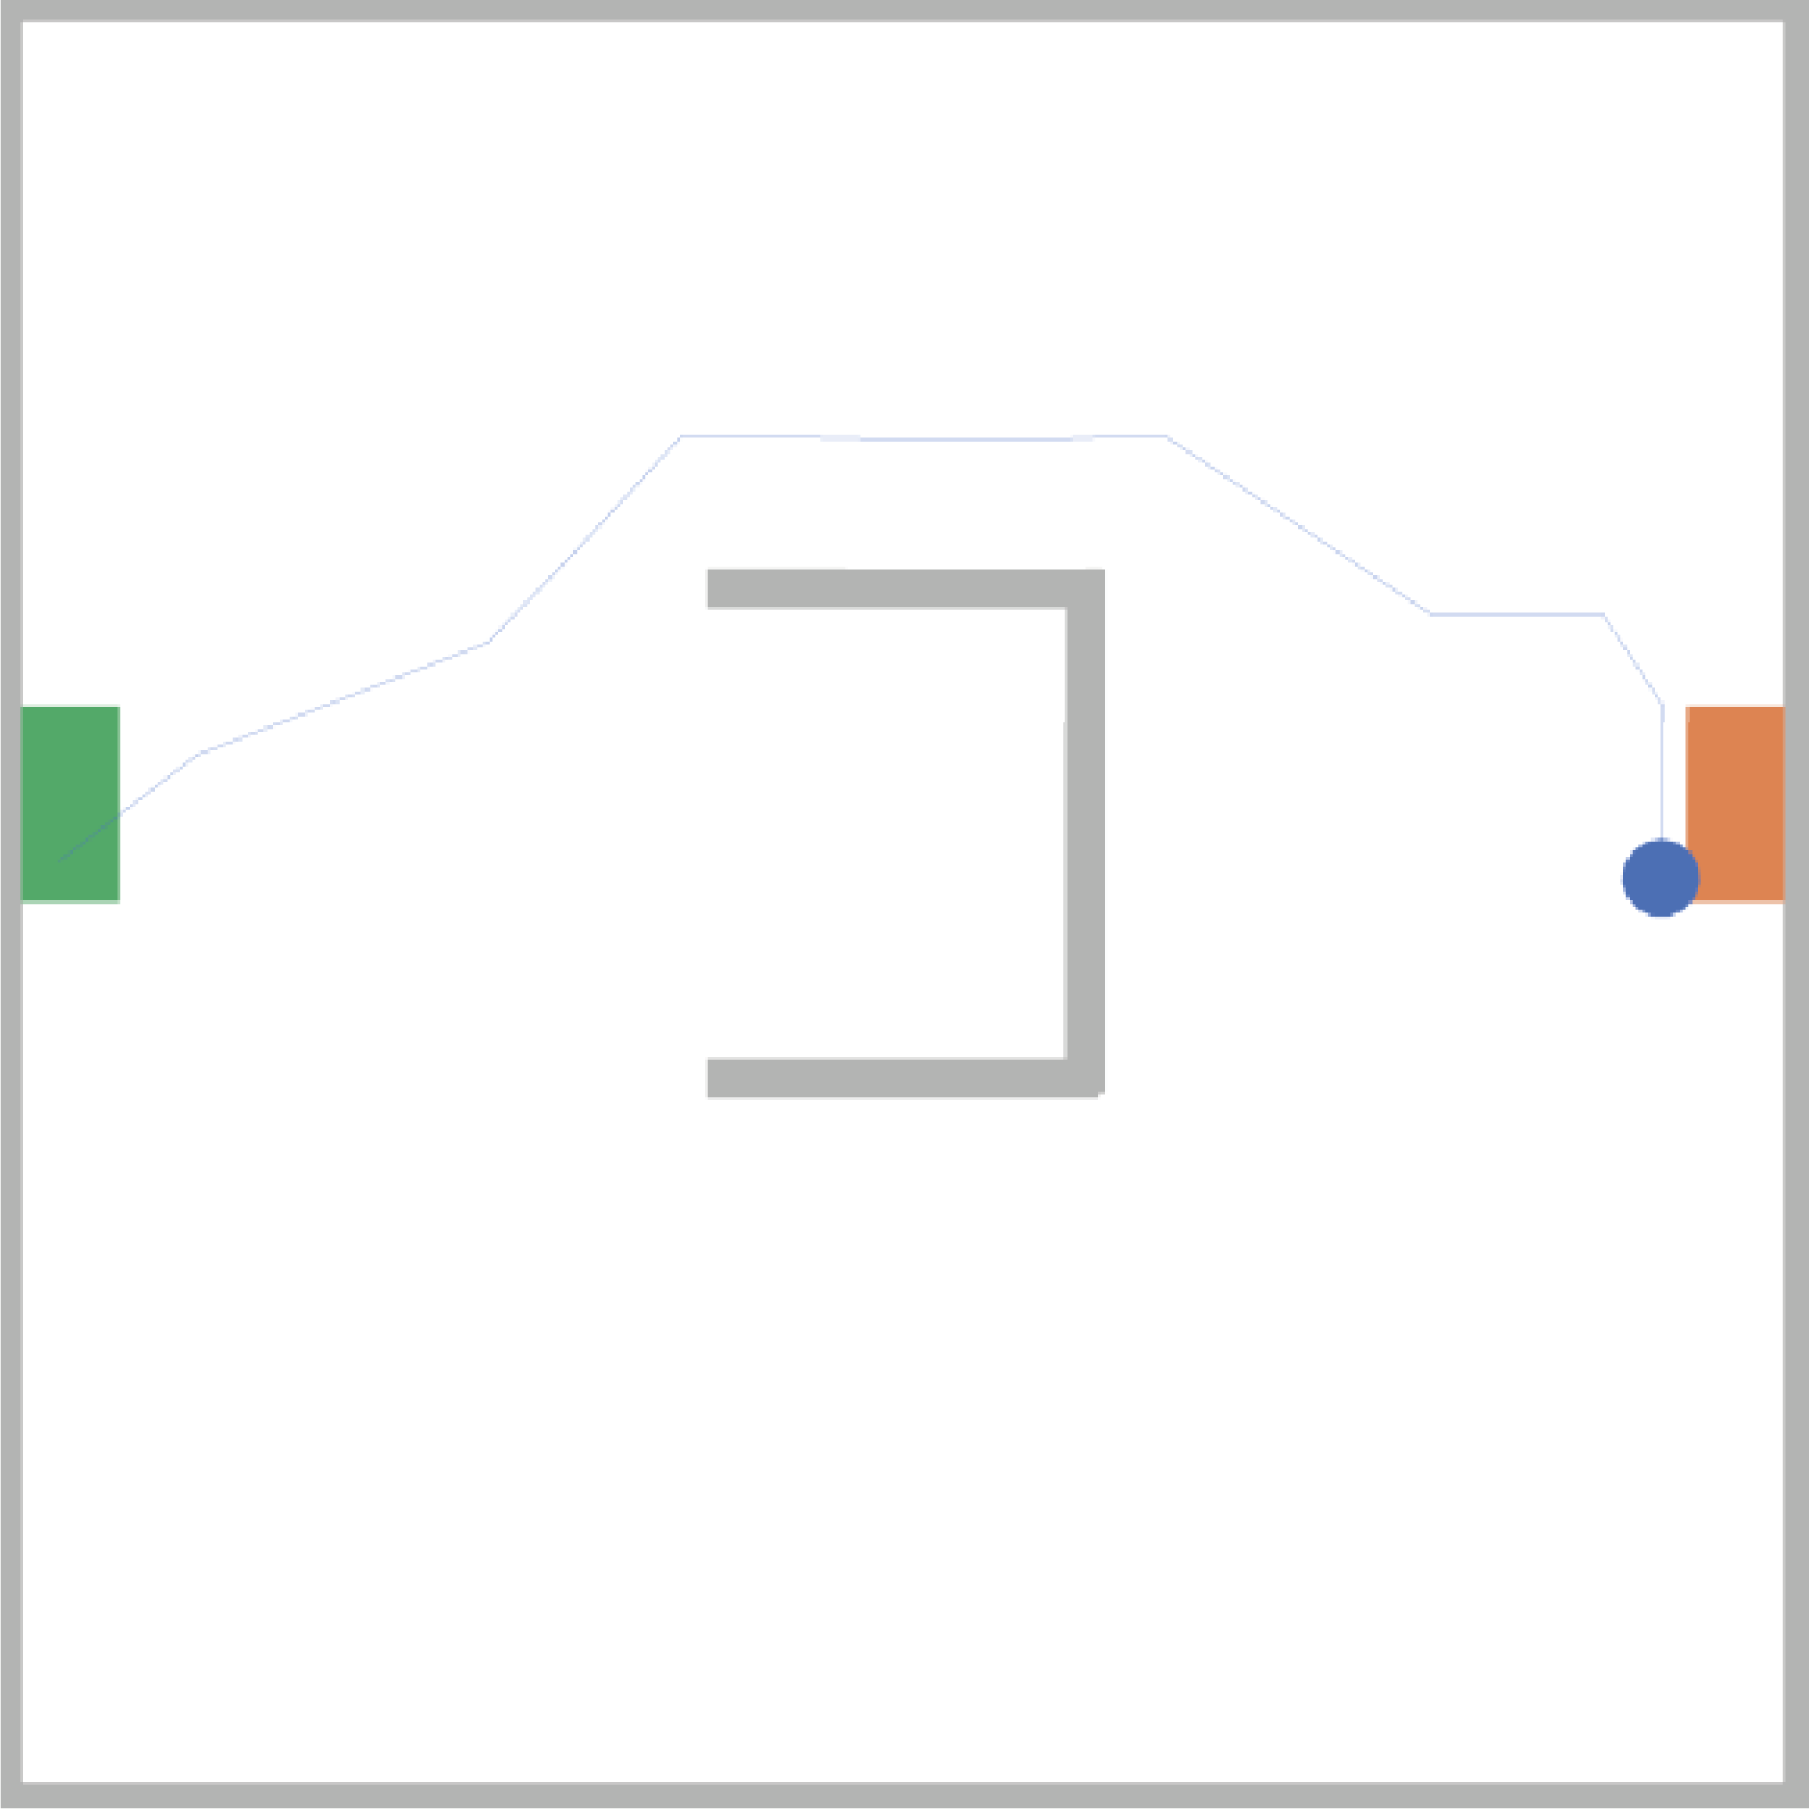
\includegraphics[width=\textwidth]{images/2-osm-chicken.png}
    \caption{Optimal Step Model}
    \label{fig: chicken-osm}
 \end{subfigure}
 \begin{subfigure}[b]{0.3\textwidth}
      \centering
     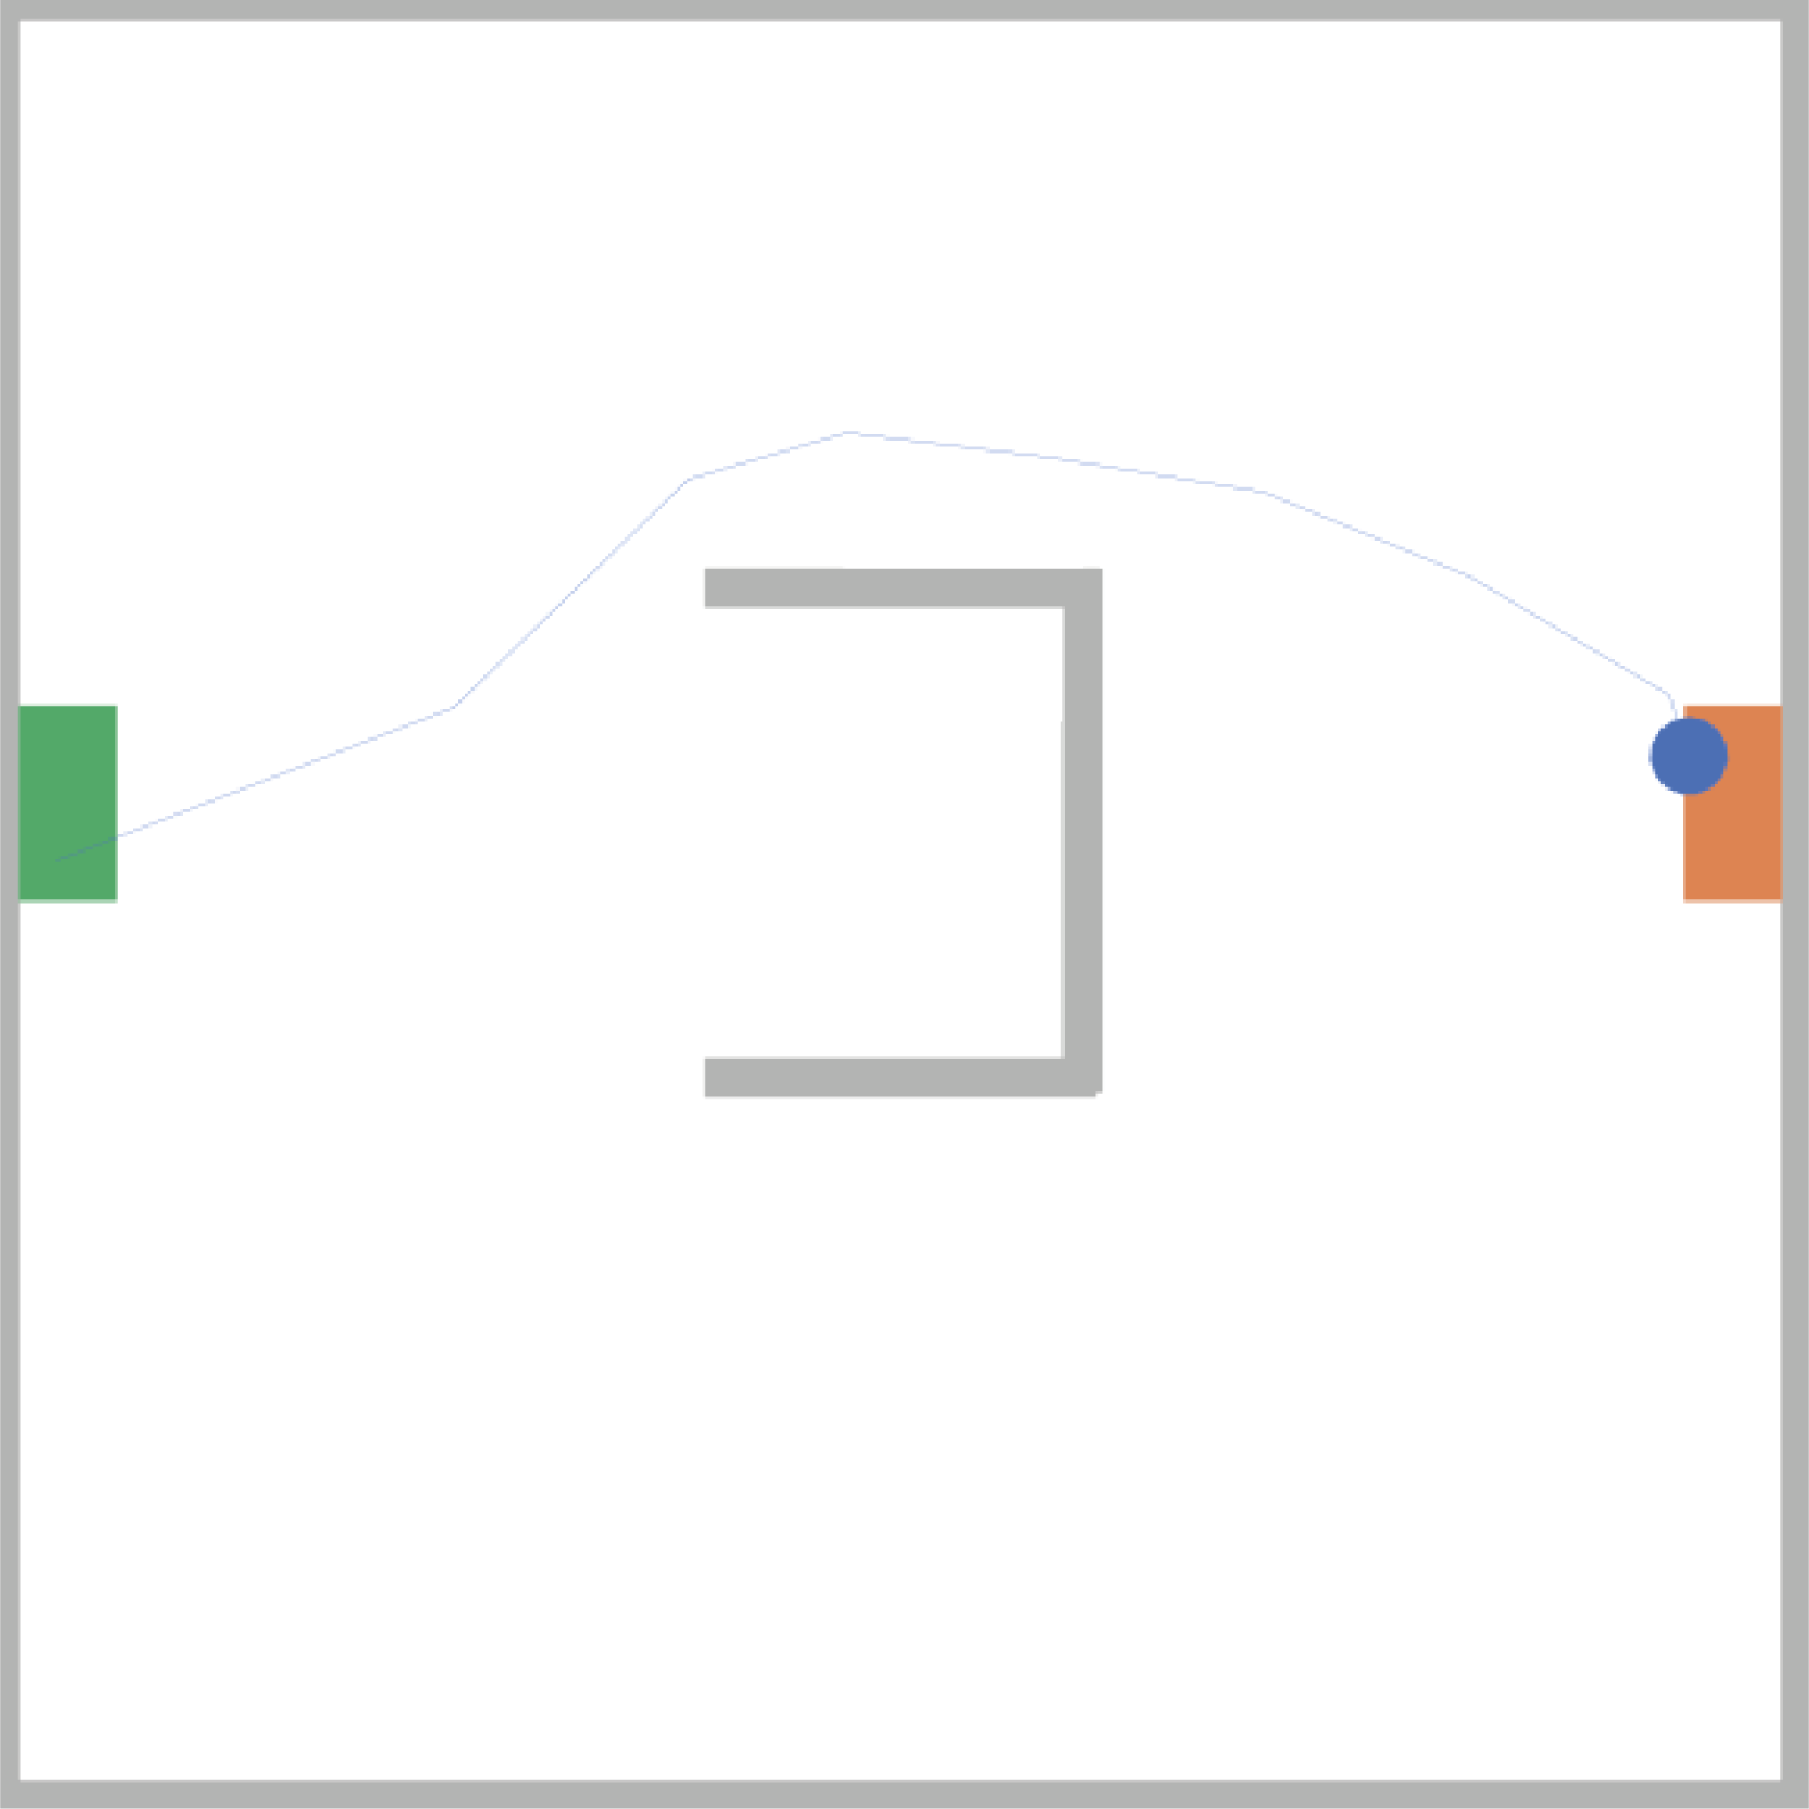
\includegraphics[width=\textwidth]{images/2-sfm-chicken.png}
     \caption{Social Force Model}
     \label{fig: chicken-sfm}
 \end{subfigure}
 \begin{subfigure}[b]{0.3\textwidth}
      \centering
     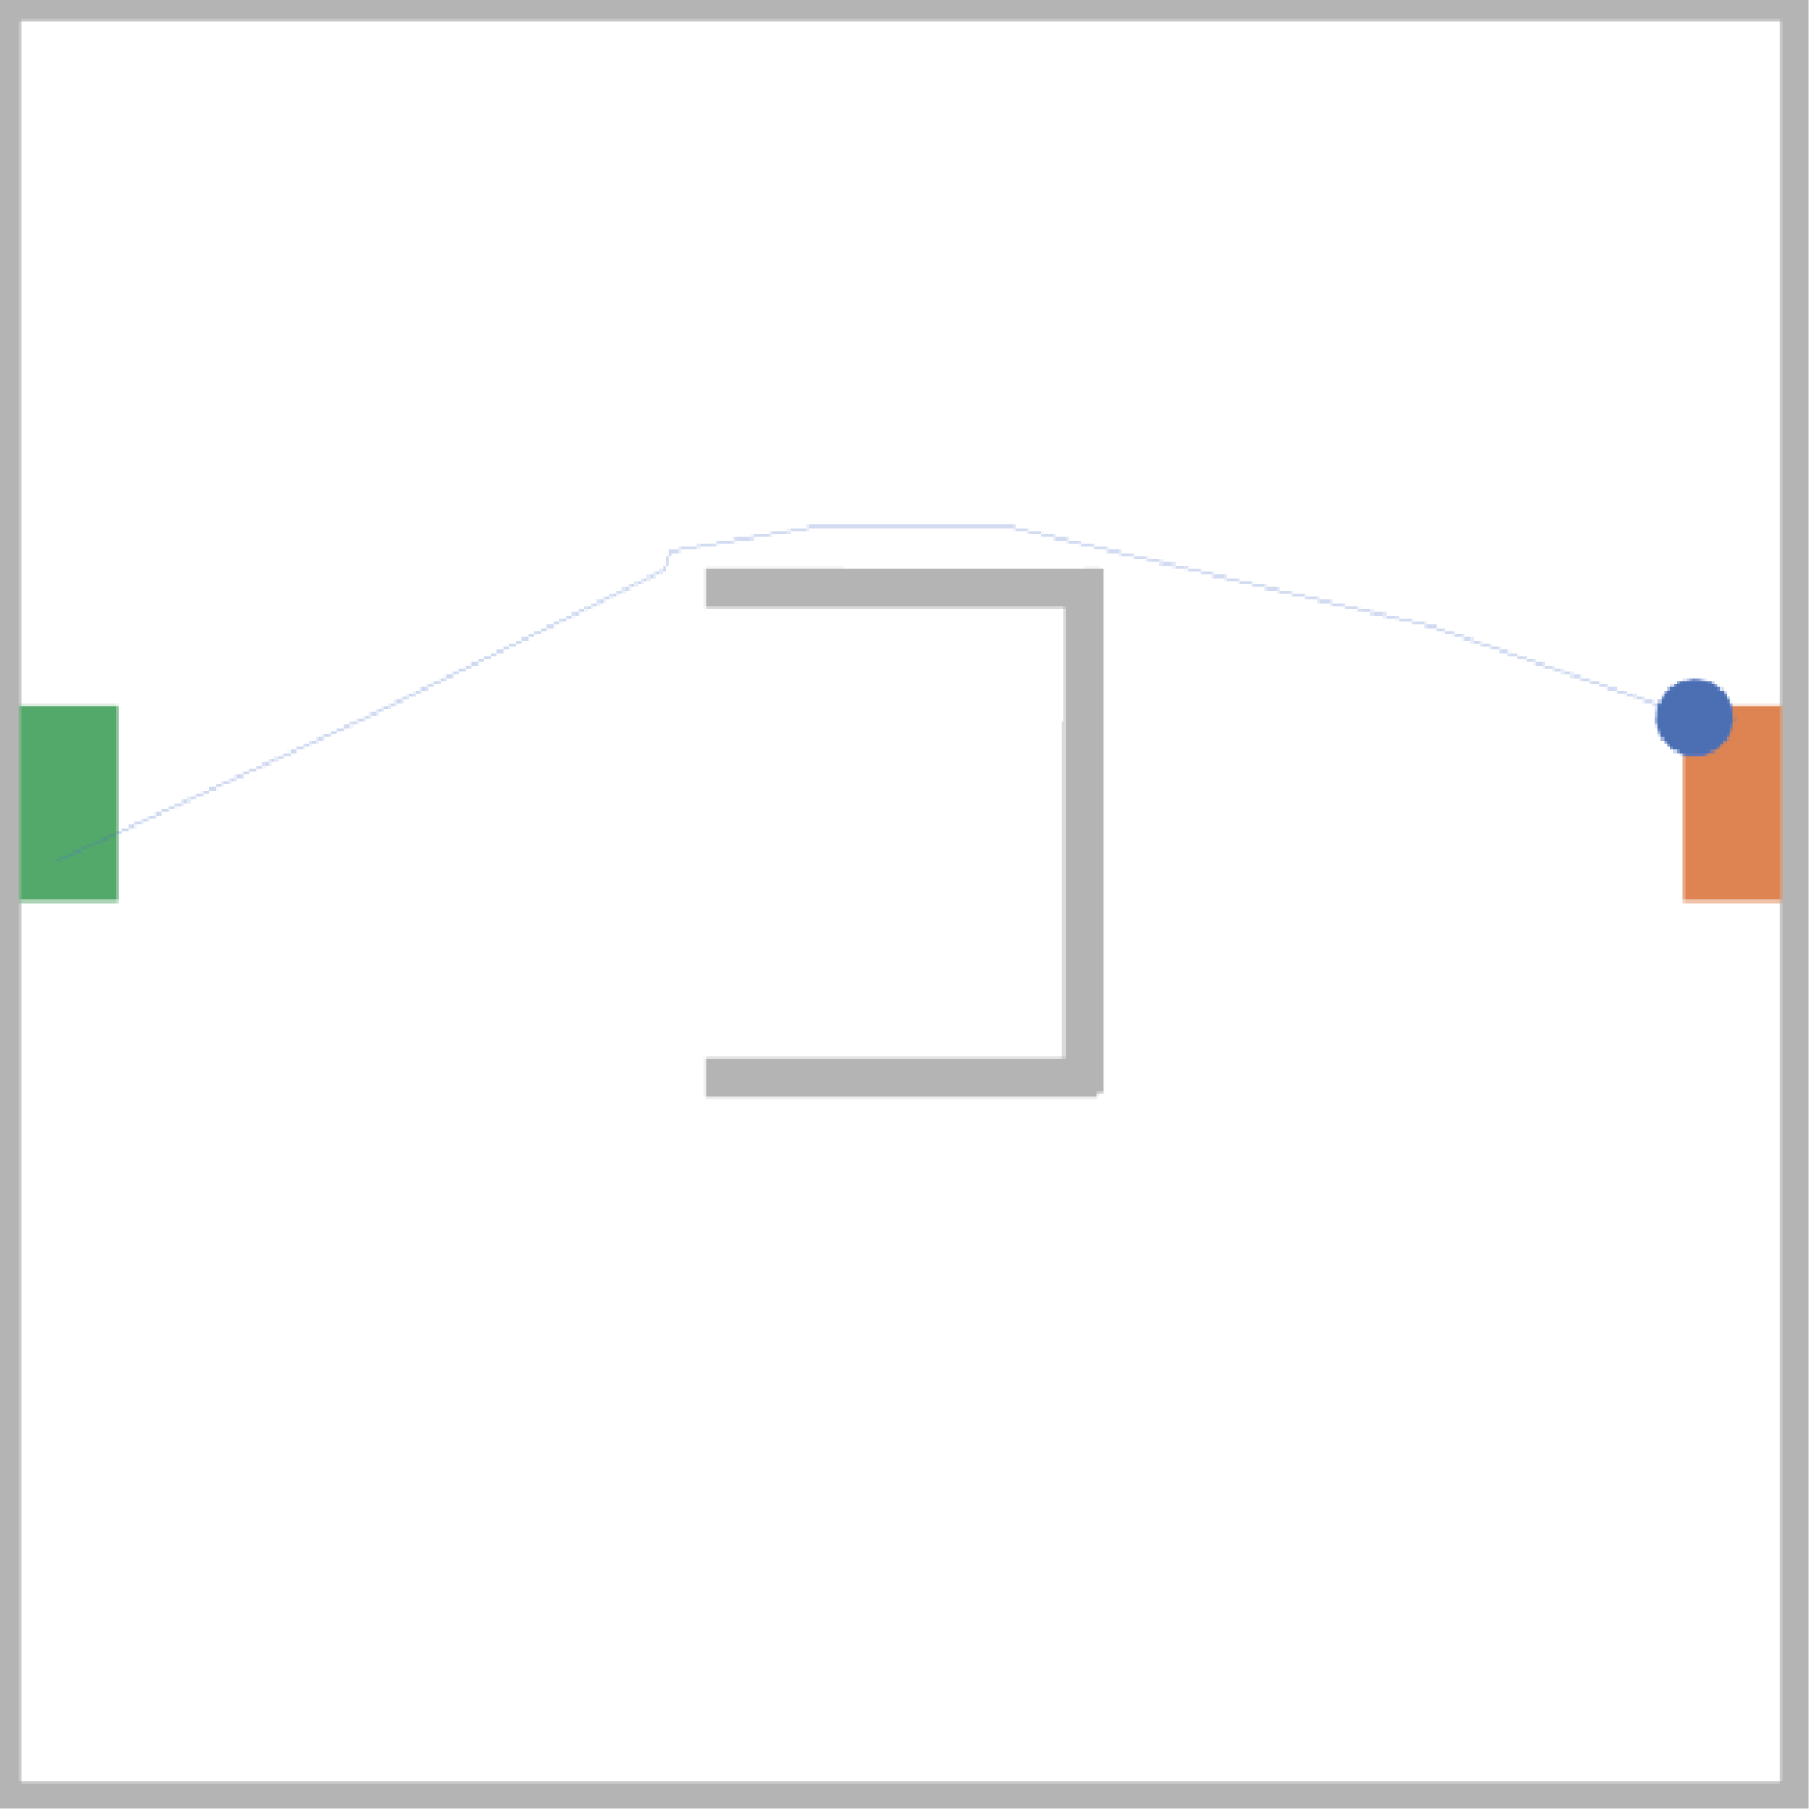
\includegraphics[width=\textwidth]{images/2-gnm-chicken.png}
     \caption{Gradient Navigation Model}
     \label{fig: chicken-gnm}
 \end{subfigure}
 \caption{Chicken Test using different models}
 \label{fig: chicken-task2}
\end{figure}